\documentclass[11pt,a4paper]{article}
\usepackage[utf8]{inputenc}
\usepackage{amsfonts}
\usepackage{pdfpages}
\usepackage{eurosym}
\usepackage{pgfplots}
\usepackage{authblk}
\usepackage{url}
\usepackage{multirow}
\usepackage{booktabs}
\usepackage{float}
\usepackage{listings}

\usepackage{hyperref}
\hypersetup{
    colorlinks=true,
    linkcolor=black,
    filecolor=magenta,      
    urlcolor=cyan,
    pdftitle={Overleaf Example},
    pdfpagemode=FullScreen,
    }
\usepackage{algpseudocode}
\usepackage{algorithm}
\usepackage{letltxmacro}
\usepackage{microtype}
\usepackage[left=3cm,right=3cm,bottom=3.5cm]{geometry}
\usepackage{emptypage}
\usepackage{amsmath,amssymb,amsthm, latexsym}
\usepackage[english,italian]{babel}
\usepackage{url}
\usepackage{caption}
\usepackage{verbatim}
\captionsetup{tableposition=top,figureposition=bottom,font=small,format=hang,labelfont={sf,bf}}
\usepackage{graphicx}
\usepackage{tabularx}
\usepackage{listings}
\usepackage{hyphenat}
\usepackage{subfig}
\pagestyle{empty}
\newcommand\AlCentroPagina[1]{%
\AddToShipoutPicture*{\AtPageCenter{%
\makebox(0,0){\includegraphics%
[width =0.9\paperwidth]{#1}}}}}

\begin{document}
\newcommand{\horrule}[1]{\rule{\linewidth}{#1}}
\lstset{language=Java} 
\lstset{basicstyle=\footnotesize\ttfamily}
\author{Silvio Baratto, Tobias Ganzmann}
\title{
\normalfont \normalsize 
\href{https://github.com/SilvioBaratto/Numerical-and-Data-Intensive-Computing}{github.com/SilvioBaratto/Lab-1} \\ [25pt] % Your university, school and/or department name(s)
\horrule{0.5pt} \\[0.4cm] % Thin top horizontal rule
\huge Report Lab 1\\ % The assignment title
\horrule{2pt} \\[0.5cm] % Thick bottom horizontal rule
}
\maketitle
\tableofcontents
\newpage
\section{PERF (I)}
\subsection{Definition profiler}
A profiler in software engineering, is a form of dynamic program analysis that measures, for example, the space (memory) or time complexity of a program, the usage of particular instructions, or the frequency and duration of function calls. Most commonly, profiling information serves to aid program optimization, and more specifically, performance engineering. Profilers, which are also programs themselves, analyze target programs by collecting information on their execution. Based on their data granularity, on how profilers collect information, they are classified into event based or statistical profilers.\\
\subsection{Code explanatin for benchmarking}
The code given to do some performance analysis using perf as a profiler consist in a simple function that initialize a matrix of dimension $2000 \times 2000$ and fill all the matrix with a value equal to $1$. The program repeat this operation $100$ times. 
\subsection{Performance analysis tool (perf)}
We are interested in see how the program behaves with different optimizers and code optimizations using perf to check the performance results. To do that with this instructions we want to look at:
\begin{itemize}
\item[\textbf{a.}] CPU clock cycles at user level
\item[\textbf{b.}] Machine code instructions at user level
\item[\textbf{c.}] First-level data cache load hitst at user level
\item[\textbf{d.}] First-level data cache load misses at user level
\item[\textbf{e.}] First-level data cache store hits at user level
\item[\textbf{f.}] First-level data cache store misses at user level
\item[\textbf{g.}] Last-level cache load hits at user level
\item[\textbf{h.}] Last-level cache load misses at user level
\item[\textbf{i.}] Last-level cache store hits at user level
\item[\textbf{j.}] Last-level cache store misses at user level
\end{itemize}
The way how we obtain the following benchmark results is from this terminal command:
\begin{lstlisting}[language=bash]
  $ sudo perf stat -e cycles:u -e instructions:u \
                	-e L1-dcache-loads:u -e L1-dcache-load-misses:u \
                	-e L1-dcache-stores:u -e L1-dcache-store-misses:u \
                	-e LLC-loads:u -e LLC-load-misses:u \
                	-e LLC-stores:u -e LLC-store-misses:u ./task1 
\end{lstlisting}
From the first run of the code we obtain the following results:
\begin{lstlisting}[language=bash]
CPU = 5.893150 ms 

 Performance counter stats for './task1':

     2,743,735,005      cycles:u         	  (32.74%)
     3,199,246,694      instructions:u            (44.26%)
       402,366,995      L1-dcache-loads           (55.79%)
       803,099,963      L1-dcache-load-misses     (67.31%)
       799,527,269      L1-dcache-stores          (67.46%)
   <not supported>      L1-dcache-store-misses                                      
         1,628,527      LLC-loads                 (67.46%)
             1,094      LLC-load-misses           (44.21%)
         2,479,174      LLC-stores                (21.69%)
               258      LLC-store-misses          (21.69%)

       0.590644181 seconds time elapsed

       0.590584000 seconds user
       0.000000000 seconds sys
\end{lstlisting}
Changing the code in such way that array is now traversed by rows
instead of by columns, hence taking advantage of both the row major order used in C and the cache hierarchy we obtain the following results:
\begin{lstlisting}[language=bash]
CPU = 1.423880 ms 

 Performance counter stats for './task1':

       648,114,804      cycles:u                  (32.97%)
     1,624,440,721      instructions:u            (44.14%)
       396,820,828      L1-dcache-loads           (55.31%)
        12,204,130      L1-dcache-load-misses     (66.48%)
       383,946,246      L1-dcache-stores          (66.48%)
   <not supported>      L1-dcache-store-misses                                      
             1,680      LLC-loads                 (66.48%)
                40      LLC-load-misses           (44.69%)
         6,988,534      LLC-stores                (22.35%)
                67      LLC-store-misses          (22.35%)

       0.143955657 seconds time elapsed

       0.135983000 seconds user
       0.007999000 seconds sys
\end{lstlisting}
From the graph below we can see how much changing to the row major perform better on cycles, instructions and cache. 
\subsection{Conclusion}
\newpage
\section{PERF (II)}
\newpage
\section{GPROF}
\begin{itemize}
\item[a] Functions with high "self ms/call" (shown in green) values and a big percentage of running time are considered our bottlenecks. The cannot be divided into smaller pieces and therefore not be parallelized.
\item[b] In contrast, functions with low "self ms/call" (shown in blue) values and frequent calls are already divided up in small, very managable chunks and can therefore be parallelized. In this case we divide the matrices in chunks and loop over them seperately in parallel (for example domain decomposition).
\end{itemize}
\begin{center}
\begin{figure}[h]
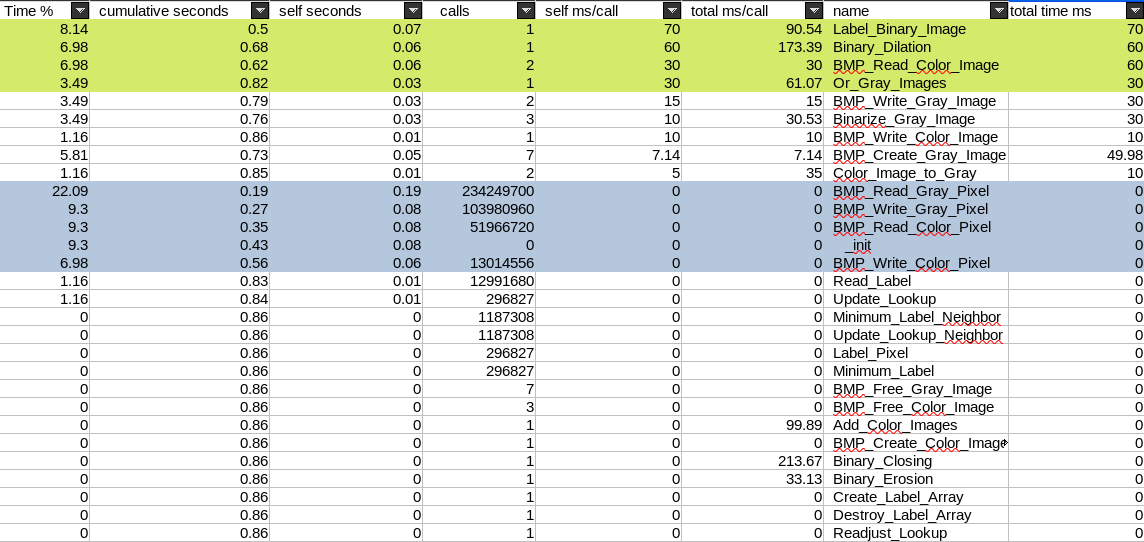
\includegraphics[width=\textwidth]{calls.png}
\end{figure}
\end{center}
\newpage
\section{OpenMP (Compilation and basic directives)}

\newpage
\section{Optional assignment}
\end{document}